\documentclass[12pt]{article}
\usepackage[utf8]{inputenc}
\usepackage{mathpartir}
\usepackage{graphicx}
\graphicspath{ {./images/} }

\begin{filecontents}{refs.bib}
@inproceedings{aam,
  title={Abstracting abstract machines},
  author={Van Horn, David and Might, Matthew},
  booktitle={Proceedings of the 15th ACM SIGPLAN international conference on Functional programming},
  pages={51--62},
  year={2010}
}
\end{filecontents}

\title{CS4215 Project Report \\\ \\\
Team Estepona - Abstract Abstract Machines}

\author{Tay Jing Xuan \and Tee Weile Wayne}
\date{April 2022}

\begin{document}

\maketitle

\section{Abstract}
We implemented an abstract interpreter for a subset of source. By approximating program states, our abstract interpreter always terminates and can be used to analyse program behaviour and allow for code optimisation. Our interpreter also allows for visualisation of the abstract state-space for analysis.

\section{Introduction}
The objective of static program analysis is to determine the behaviour of a program without running it. This includes determining whether the program terminates, whether optimisations can be applied, and what states are reachable during program execution.

This is a difficult problem. The halting problem for example is undecidable. Data-flow analysis is also difficult to perform on languages such as Source which support higher-order functions.

A key difficulty is that a virtual machine executing a program might require an infinite number of states for a non-terminating program. However, by following the abstracting abstract machines approach \cite{aam}, we are able to convert a concrete virtual machine into a non-deterministic abstract machine with finite states, with each abstract state representing multiple possible concrete states. As a result, we are able to soundly approximate program behaviour in finite time.

For example, if the concrete machine transitions from state $A$ to state $B$, then the abstract machine must transition from some abstract state $A^{\prime}$ to some abstract state $B^{\prime}$, where $A^{\prime}$ and $B^{\prime}$ are the abstract states representing $A$ and $B$. If the abstract machine always terminates, then so must the concrete machine.

We applied this approach to convert the Source virtual machine into an abstract interpreter which supports higher-order functions and conditionals. The interpreter provably terminates, returning a graph of abstract states reached that can be visualised by the user and potentially used to derive complier optimisations.

\section{Implementation}
\subsection{Overview}
Our abstract interpreter runs on the Source virtual machine code produced by the Source complier. We derived it from the original Source virtual machine by applying the technique of abstracting abstract machines \cite{aam}. Each state of our abstract interpreter is of the form:
$$(PC,OS,ENV,STORE,KONT,TIME,C)$$

Similar to the original Source virtual machine, $PC$ is a number representing the program counter and $OS$ is the operand stack itself, storing integers, booleans and closures. $ENV$ maps the names of function parameters and local variables to addresses. Note that these names in practice are actually integers. $STORE$ maps addresses to values. $KONT$ is the address of the continuation. A continuation is similar to a stack frame and it stores the previous $PC,OS,ENV,KONT,TIME$ and $C$. $TIME$ is a string representing the current call stack. It is the concatenation of the locations of the $CALL$ instructions in the call stack and is used to allocate new addresses. $C$ is an incrementing counter that is used alongside $TIME$ to allocate new addresses.

Note that all the rules below increment the $PC$ by 1 to advance to the next instruction. In actual implementaion, a single instruction may take up multiple slots, hence incrementing by more than 1 may be necessary.

\subsection{Store}
Importantly, the $STORE$ maps each address (a string) to a set of values. When the store is dereferenced by any instruction, the interpreter non-deterministically chooses a value from the set of possible values, and transitions to the corresponding new state. When generating the state graph, all such possible transitions are explored.

To illustrate, here are the rules for the load and assignment instructions:

$$\infer{s(PC) = LD\ name}{
    (PC,OS,ENV,STORE,KONT,TIME,C) \rightarrow \\
    (PC+1,v.OS,ENV,STORE,KONT,TIME,C)}$$
where $v \in STORE(ENV(name))$

$$\infer{s(PC) = ASSIGN\ name}{
  (PC,v.OS,ENV,STORE,KONT,TIME,C) \rightarrow \\
  (PC+1,OS,ENV,STORE[ENV(name) \leftarrow v],KONT,TIME,C)}$$
where $STORE[addr \leftarrow v]$ denotes adding the value $v$ to the set of values at the address $addr$ in the $STORE$

\subsection{Functions}
\subsubsection{LDF}
The $LDF$ instruction pushes a closure on the operand stack. It receives the function address and the number of slots the environment needs to be extended by (number of parameters and local variables) as input.

$$\infer{s(PC) = LDF\ \ funcAddr\ \ numToExtend}{
    (PC,OS,ENV,STORE,KONT,TIME,C) \rightarrow \\
    (PC+1,closure.OS,ENV,STORE',KONT,TIME,C)}$$
where
$$envAddr=TIME.funcAddr.``env''$$
$$STORE'=STORE[envAddr \leftarrow ENV]$$
$$closure=(funcAddr,envAddr,numToExtend)$$

Note that the environment address is the $TIME$ concatenated with the function address concatenated with the string constant $``env''$. The use of the function address and string constant ensures that the set of values stored at this address are all environnments which are compatible with this function.

\subsubsection{CALL}
The $CALL$ instruction is more complex. It receives the number of parameters as input, and pops the the parameters and closure from the operand stack. Afterwards, it extends the function environment in the closure, saves the current state as a continuation, and transitions to the new function.

$$\infer{s(PC) = CALL\ \ n}{
    (PC,OS,ENV,STORE,KONT,TIME,C) \rightarrow \\
    (PC',(),ENV',STORE',KONT',TIME',0)}$$
where
$$OS=V_n...V_2.V_1.closure.OS'$$
$$closure=(PC',funcEnvAddr,numToExtend)$$

$$funcEnv \in STORE(funcEnvAddr)$$
$$s=|funcEnv|$$
$$ENV'=funcEnv[s+1 \leftarrow A_1]...[s+numToExtend \leftarrow A_{numToExtend}]$$
$$STORE_1=[A_1 \leftarrow V_1]...[A_n \leftarrow V_n]$$
$$A_i=alloc(TIME,C+i) \quad where\ 0 \leq i < numToExtend$$

$$kontAddr = TIME.PC.``kont''$$
$$envAddr = kontAddr.``env''$$
$$osAddr = kontAddr.``os''$$
$$STORE_2=STORE_1[envAddr \leftarrow ENV]$$
$$STORE_3=STORE_2[osAddr \leftarrow OS]$$
$$STORE'=STORE_3[kontAddr \leftarrow kontObj]$$
$$kontObj = (PC+1,osAddr,envAddr,KONT,TIME,C+numToExtend)$$
$$KONT' = kontAddr$$

$$TIME' = truncate(TIME.PC)$$

Note that the names added to the environment are in the range $s+1$ to $s+numToExtend$ where $s$ is the original size of the environment. Also note this rule can be applied with $funcEnv$ being any of the environments stored in the store under that particular address. The addresses are allocated by the $alloc$ function that takes in the $TIME$ and counter $C$ and returns the address $TIME.``v''.C$. The string constant $``v''$ denotes that these addreses are meant to store values.

The $CALL$ instruction also stores the current $ENV$, $OS$ and other parameters in the state as part of a continuation object. $KONT'$ is the address pointing to this object and the format of the address includes the current $PC$ which ensures that all possible continuations stored in this address returns to this $PC$. In other words, this ensures that no two continuations returning to different places exists in the same address in the store.

Finally the value of $TIME'$ is created by appending the current $PC$ to the current $TIME$ then trucating it if necessary to a predefined maximum length of $MAX\_TIME$. This is necessary to ensure that the abstract interpreter terminates, which we will prove in the analysis section.

\subsubsection{RTN}
The $RTN$ function returns a value to any of the continuations stored at the address $KONT$.

$$\infer{s(PC) = RTN}{
    (PC,v.OS,ENV,STORE,KONT,TIME,C) \rightarrow \\
    (PC',v.OS',ENV',STORE,KONT',TIME',C')}$$

where
$$(PC',osAddr,envAddr,KONT',TIME',C') \in STORE(KONT)$$
$$OS' \in STORE(osAddr)$$
$$ENV' \in STORE(envAddr)$$

\subsection{Bounding of values}
To ensure that states are finite, values of numbers are bounded by the constants $MIN\_NUM$ and $MAX\_NUM$, numbers which exceed these bounds during runtime will be replaced with the constant $``unum''$, representing an unknown number. Arithmetic operations involving $``unum''$ will result in $``unum''$. Evaluating expressions such as $``unum'' > 0$ will result in the constant $``ubool''$. The conditional instruction $JOF$ can non-deterministically jump to either address when applied to $``ubool''$.

\subsection{Execution}
The abstract interpreter receives a Source program as input. It then compiles it into Source virtual machine code. Starting with the state:
$$(0,(),\emptyset,\emptyset,``'',``0'',0)$$
It applies the rules above using depth-first search to explore all possible states. These states are then returned to the user and can be visualised as a graph.

\section{Analysis}
To correctness of our abstract interpreter, we now prove soundness and decidability.

\subsection{Soundness}
To show soundness, we have to show that if the concrete machine transitions from state $A$ to state $B$, then the abstract machine must transition from some abstract state $A^{\prime}$ to some abstract state $B^{\prime}$. Where $A^{\prime}$ and $B^{\prime}$ are the abstract versions of $A$ and $B$.

There are two important differences between the abstract states and the concrete states. These are ways in which the abstract machine approximates the concrete one.

Firstly, the abstract machine deals with bounded numbers, using the constants ``unum'' and ``ubool'' to represent any number and boolean. Numbers and booleans in the concrete state may be replaced by these unknown values in the abstract. This does not compromise soundness.

Secondly, each address in the abstract machine points to a set of values instead a single value. Another way of seeing this is that values in the concrete store may have to ``share'' an address in the abstract store. For all semantic rules of the concrete machine, the abstract version of the rule accounts for all possible values when dereferencing the store. Hence all of the state transitions in the concrete machine must be represented by a state transistion in the abstract. Hence soundness is preserved here as well.

\subsection{Decidability}
To show decidability, we show that the number of states is finite. 
\begin{itemize}
  \item $PC$ is bounded by the size of the compiled program, which is finite.
        
  \item $TIME$ is a string truncated to a constant length.
        
  \item $C$ is finite as it is only incremented by the $CALL$ instruction, and as the number of function calls and the sizes of their environments are finite.
        
  \item Addresses are created only by the $LDF$ and $CALL$ instuctions. They are bounded by $TIME$, the program size, and $C$ which are all finite.
        
  \item Closures include the $PC$ of the function, the address of its environment and the number of local variables and parameters, all of which are finite.
        
  \item $OS$ is of finite size (as guaranteed by compiler), storing values which includes bounded numbers, booleans, and closures. Hence number of possible $OS$ is finite.
        
  \item $ENV$ is finite as names and and addresses are finite.
        
  \item $KONT$ is finite as it is an address.
        
  \item Continuations are finite as they store addresss, counters and $TIME$, which are finite.
        
  \item $STORE$ is finite as as addreses are finite, and it stores bounded numbers, booleans, closures, operand stacks, environments and continuations, all of which are finite.
\end{itemize}

This shows that there are finite states, as each state is evaluated once, the abstract interpreter terminates. This proves decidability.

\section{Results}
\subsection{Simple Example}
We now demonstrate our interpreter on a simple, non-terminating program with $MAX\_TIME$ set to 3:

\begin{verbatim}
  function f(){
    return f();
  }
  f();
\end{verbatim}
Compiling the program results in the following machine code. Note that we have modified the compiler to retain function and variable names.

\begin{verbatim}
  0: START
  1: LDF 1 8 1
  5: CALL 0
  7: DONE
  8: LDF 1 21 0
  12: ASSIGN [0, "f"]
  14: LDCU
  15: POP
  16: LD 0
  18: CALL 0
  20: RTN
  21: LD 0
  23: CALL 0
  25: RTN
\end{verbatim}
Applying our abstract interpreter results in a finite number of states ending with a loop as shown:
\begin{center}
  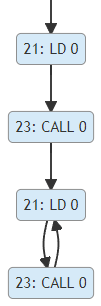
\includegraphics[scale=0.7]{simple_graph.png}
\end{center}
The second last state from the bottom is shown here:
\begin{small}
  \begin{verbatim}
PC:	  21
TIME:	0.5.18
OS:	  []
KONT:	0.5.18.23.kont
ENV:	 [0 -> 0.v1]
STORE:
0.8.env -> []
0.5.kont.env -> []
0.5.kont.os -> []
0.5.kont -> [7,"0.5.kont.os","0.5.kont.env","","0",1]
0.5.21.env -> [[0,"0.v1"]]
0.v1 -> ["CLOSURE",21,"0.5.21.env",0]
0.5.18.kont.env -> [[0,"0.v1"]]
0.5.18.kont.os -> []
0.5.18.kont -> [20,"0.5.18.kont.os","0.5.18.kont.env","05.kont","0.5",0]
0.5.18.23.kont.env -> [[0,"0.v1"]]
0.5.18.23.kont.os -> []
0.5.18.23.kont -> 
 [25,"0.5.18.23.kont.os","0.5.18.23.kont.env","0.5.18.kont","0.5.18",0] ||
 [25,"0.5.18.23.kont.os","0.5.18.23.kont.env","0.5.18.23.kont","0.5.18",0]
\end{verbatim}
\end{small}
The only difference between the last state and second last state except that the $PC$ of the last state is 23 and the $OS$ has a single entry, which is the closure \verb|[21,0.5.21.env,0]|. 

Observe that the address \verb|0.5.18.23.kont| in the store points a set of 2 continuations. When the $CALL$ instruction executes, it creates a continuation to store the current state. This continuation would be stored at the address \verb|0.5.18.23.kont|, but as the store already contains the same exact continuation at that address, the store is left unchanged. This explains why the states loop.

This looping occurs only because the $TIME$ is truncated. If $TIME$ is not truncated, each call would cause the length of $TIME$ to increase, hence there would not be a loop. Furthermore, if $TIME$ is not truncated, each continuation would have its own unique address.

Increasing the value of $MAX\_TIME$ in this example would only lead to a longer chain of states being explored before the same loop is reached.

\subsection{More Complex Example}
We now demonstrate our interpreter on a more complex program:
\begin{verbatim}
  function f(x){
    return f(x+1);
  }
  f(7);
\end{verbatim}
Setting $MAX\_TIME$ to 3 and $MAX\_NUM$ to 10 results in the following states:
\begin{center}
  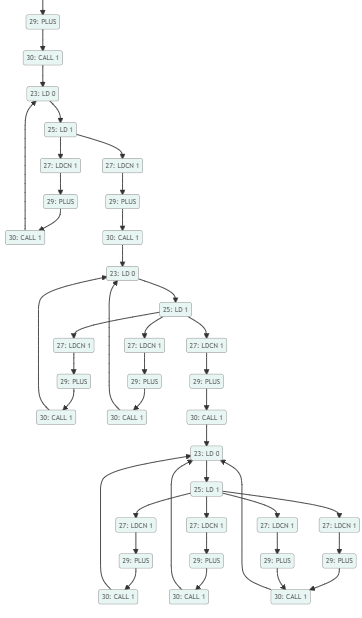
\includegraphics[scale=0.7]{complex_graph.png}
\end{center}
The interpreter terminates and the branches represent the $LD$ instruction dealing with multiple possible values of x in the store (8, 9, 10 and ``unum'').

\bibliography{refs}
\bibliographystyle{plain} % We choose the "plain" reference style

\end{document}

